\section{Algorithme génétique}
L'algorithme génétique\cite{GenCNN} est une méthode bio-inspirée ressemblant à la sélection naturelle. Cette approche évolutionnaire permet d'explorer efficacement l'espace de recherche des architectures de réseaux de neurones en appliquant les principes de sélection, croisement et mutation, sur une population d'individus représentant différentes architectures. L'avantage principal de cette méthode réside dans sa capacité à échapper aux optima locaux grâce à la diversité maintenue dans la population et aux opérateurs stochastiques qui permettent d'explorer des régions prometteuses de l'espace de recherche.



\subsection{Représentation de l'espace de recherche}
La représentation des architectures constitue un élément fondamental dans l'efficacité d'un algorithme génétique. Dans notre approche, chaque architecture de réseau de neurones convolutionnel est encodée sous forme de chaîne binaire, permettant une manipulation directe et efficace lors des opérations génétiques.
\subsubsection{Encodage binaire des architectures}
Chaque couche du réseau est représentée par un chromosome de longueur fixe de 8 bits, structuré de manière hiérarchique. Les deux premiers bits définissent le type de couche selon le codage suivant :
\begin{itemize}
\item \texttt{00} : absence de couche (position vide dans l'architecture)
\item \texttt{01} : couche convolutionnelle
\item \texttt{10} : couche de sous-échantillonnage (pooling)
\item \texttt{11} : couche entièrement connectée
\end{itemize}
Les six bits restants encodent les paramètres spécifiques à chaque type de couche. Pour les couches convolutionnelles, ces paramètres comprennent le nombre de filtres, la taille du noyau de convolution et le pas de convolution. Les couches de pooling sont caractérisées par la taille de leur fenêtre et leur pas, tandis que les couches entièrement connectées sont définies par leur nombre de neurones et leur fonction d'activation. La Figure \ref{fig:exemple d'encodage binaire} montre un exemple d'une architecture de CNN simple avec une couche de convolution, une couche de pooling et une couche entièrement connectée.

% Définition des couleurs
\definecolor{convcolor}{RGB}{52, 152, 219}
\definecolor{poolcolor}{RGB}{231, 76, 60}
\definecolor{fccolor}{RGB}{46, 204, 113}
\definecolor{nullcolor}{RGB}{149, 165, 166}
\definecolor{lightblue}{RGB}{173,216,230}
\definecolor{lightgreen}{RGB}{144,238,144}

\begin{figure}
    \centering
        \begin{center}
        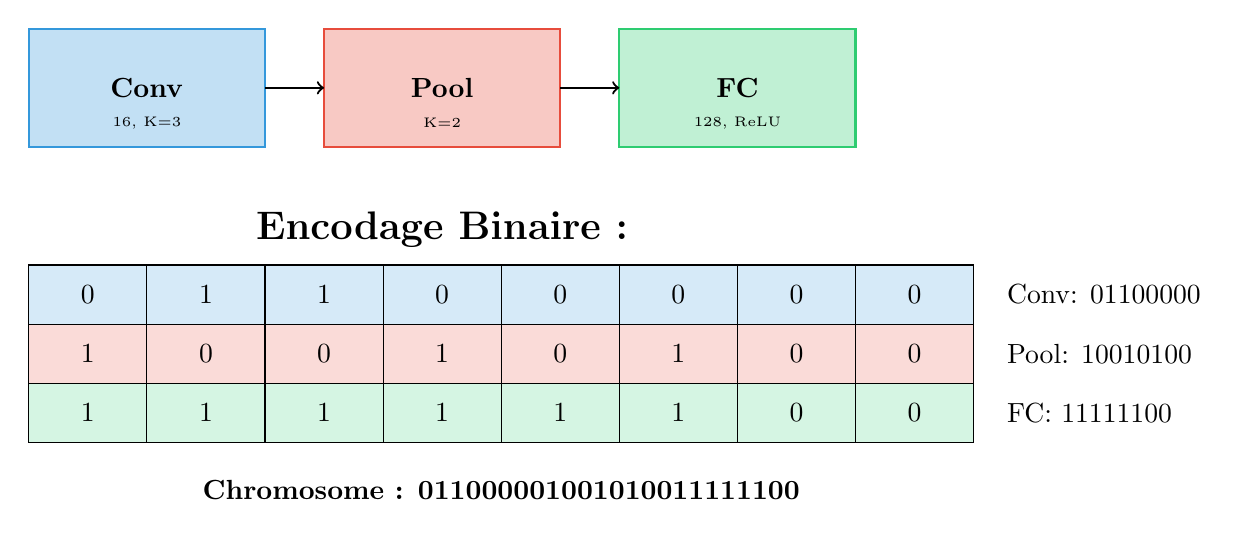
\begin{tikzpicture}[scale=1.5]
            % Architecture visuelle
            \draw[fill=convcolor!30, draw=convcolor, thick] (0,3) rectangle (2,4);
            \node at (1,3.5) {\textbf{Conv}};
            \node at (1,3.2) {\tiny 16, K=3};
            
            \draw[fill=poolcolor!30, draw=poolcolor, thick] (2.5,3) rectangle (4.5,4);
            \node at (3.5,3.5) {\textbf{Pool}};
            \node at (3.5,3.2) {\tiny K=2};
            
            \draw[fill=fccolor!30, draw=fccolor, thick] (5,3) rectangle (7,4);
            \node at (6,3.5) {\textbf{FC}};
            \node at (6,3.2) {\tiny 128, ReLU};
            
            \draw[->, thick] (2,3.5) -- (2.5,3.5);
            \draw[->, thick] (4.5,3.5) -- (5,3.5);
            
            % Encodage binaire
            \node at (3.5,2.3) {\Large \textbf{Encodage Binaire :}};
            
            % Conv : filters=16 (index 2), kernel=3 (index 0), stride=1 (index 0)
            \draw[fill=convcolor!20] (0,1.5) rectangle (8,2);
            \foreach \i/\bit in {0/0, 1/1, 2/1, 3/0, 4/0, 5/0, 6/0, 7/0} {
                \draw (\i,1.5) rectangle (\i+1,2);
                \node at (\i+0.5,1.75) {\bit};
            }
            \node[right] at (8.2,1.75) {Conv: 01100000};
            
            % Pool : kernel=2 (index ???), stride=2 (index 1)
            \draw[fill=poolcolor!20] (0,1) rectangle (8,1.5);
            \foreach \i/\bit in {0/1, 1/0, 2/0, 3/1, 4/0, 5/1, 6/0, 7/0} {
                \draw (\i,1) rectangle (\i+1,1.5);
                \node at (\i+0.5,1.25) {\bit};
            }
            \node[right] at (8.2,1.25) {Pool: 10010100};
            
            % FC : size=128 (index ???), activation=ReLU (index 0)
            \draw[fill=fccolor!20] (0,0.5) rectangle (8,1);
            \foreach \i/\bit in {0/1, 1/1, 2/1, 3/1, 4/1, 5/1, 6/0, 7/0} {
                \draw (\i,0.5) rectangle (\i+1,1);
                \node at (\i+0.5,0.75) {\bit};
            }
            \node[right] at (8.2,0.75) {FC: 11111100};
            
            % Chromosome complet
            \node at (4,0.1) {\textbf{Chromosome : 011000001001010011111100}};
        \end{tikzpicture}
        \end{center}
    \caption{Exemple d'encodage binaire d'une architecture CNN}
    \label{fig:exemple d'encodage binaire}
\end{figure}


\subsubsection{Avantages de cette représentation}
Cette représentation binaire présente plusieurs avantages significatifs. Premièrement, elle assure une longueur constante pour chaque couche, facilitant les opérations de croisement et de mutation. Deuxièmement, la séparation claire entre le type de couche et ses paramètres permet de préserver la cohérence structurelle lors des modifications. Enfin, l'utilisation d'index pour référencer les valeurs possibles des paramètres garantit que seules des configurations valides peuvent être générées.
Une architecture complète est donc représentée par la concaténation des encodages binaires de toutes ses couches, créant ainsi un génotype de longueur variable qui peut être manipulé efficacement par les opérateurs génétiques.

\subsection{Stratégies de sélection}

Dans les algorithmes évolutionnaires, la stratégie de sélection joue un rôle clé dans la pression de sélection exercée sur la population. Pour cette étude, nous avons adopter une stratégie élitiste qui consiste à choisir un nombre les $n$ meilleurs individues dans la population pour représenter la génération suivante. Néanmoins, il existe d'autre stratégie de sélection telles que la sélection par rang polynomiale\cite{4630852} qui consiste à attribuer à chaque individu une probabilité de sélection qui dépend uniquement de son rang dans la population (après tri selon la performance). Dans le cas général, on peut utiliser une fonction polynômiale de degré $d$ : 

\[
P(I = k) = \sum_{l=1}^{d+1} a_l k^{l-1}
\]

où $k$ est le rang de l’individu, et les coefficients $a_l$ sont choisis de façon à garantir que $P(I = k)$ soit toujours positive et que la somme des probabilités égale 1 sur l’ensemble de la population. Cette approche permet de moduler la pression de sélection en fonction du choix des coefficients.
Une autre stratégie de qui est la sélection par tournoi probabiliste\cite{4630852}
où on sélectionne aléatoirement $t$ individus dans la population (avec ou sans remise), puis on les classe selon leur performance. La sélection probabiliste consiste alors à choisir le $s$-ème meilleur individu du tournoi avec une probabilité $\alpha_s$ donnée. La probabilité pour qu’un individu de rang $k$ soit finalement sélectionné s’écrit alors :

\[
P(I = k) = \sum_{s=1}^t \alpha_s P(I_s = k)
\]

où $P(I_s = k)$ est la probabilité pour que l’individu de rang $k$ occupe la $s$-ème place dans le classement du tournoi.
Nous avons aussi implémenter ces deux stratégies dans notre code disponible sur github.

\subsection{Croisement}
Le croisement constitue l'opérateur principal de recombinaison génétique, permettant de combiner les caractéristiques de deux architectures parentes pour générer de nouvelles solutions potentiellement meilleures. Dans le contexte de l'évolution d'architectures de réseaux de neurones, le croisement doit préserver la cohérence structurelle tout en permettant l'émergence de nouvelles configurations.

\subsubsection{Croisement à un point adapté}
Nous avons opté pour un croisement à un point modifié, spécifiquement adapté à notre représentation binaire des architectures. Contrairement au croisement classique qui peut couper la chaîne binaire à n'importe quelle position, notre approche limite les points de coupure aux frontières entre chromosomes de couches.
Le processus se déroule comme suit : deux points de coupure sont sélectionnés aléatoirement, chacun aligné sur le début d'un chromosome de couche dans les architectures parentes respectives. Les segments suivant ces points sont alors échangés entre les parents, générant deux architectures enfants. Cette contrainte d'alignement garantit que les couches individuelles restent intactes lors du croisement.
La Figure~\ref{fig:crossover} illustre ce processus de croisement adapté. Chaque architecture parente est représentée par une séquence de chromosomes de 8 bits, où chaque chromosome encode une couche spécifique. Les points de coupure (indiqués par les flèches) sont positionnés au début des chromosomes, préservant ainsi l'intégrité de chaque couche lors de l'échange des segments.
\begin{figure}[h]
\centering
\begin{tikzpicture}[scale=1.2]
% Parent 1
\node at (-0.8, 3) {\textbf{Parent 1:}};
\foreach \i in {0,1,2,3,4} {
    \draw[fill=lightblue] (\i*1.5, 2.5) rectangle (\i*1.5+1.2, 3.5);
    \node at (\i*1.5+0.6, 3) {\footnotesize Couche \i};
}
% Encoding bits for Parent 1
\node at (0.6, 2.2) {\tiny 01110010};
\node at (2.1, 2.2) {\tiny 10010100};
\node at (3.6, 2.2) {\tiny 01001101};
\node at (5.1, 2.2) {\tiny 11001010};
\node at (6.6, 2.2) {\tiny 11010010};

% Cut point 1
\draw[red, thick, ->] (3, 4) -- (3, 3.5);
\node[red] at (3, 4.3) {\footnotesize Point de coupure};

% Parent 2
\node at (-0.8, 1) {\textbf{Parent 2:}};
\foreach \i in {0,1,2,3,4} {
    \draw[fill=lightgreen] (\i*1.5, 0.5) rectangle (\i*1.5+1.2, 1.5);
    \node at (\i*1.5+0.6, 1) {\footnotesize Couche \i};
}

% Encoding bits for Parent 2
\node at (0.6, 0.2) {\tiny 10001110};
\node at (2.1, 0.2) {\tiny 01101001};
\node at (3.6, 0.2) {\tiny 11000111};
\node at (5.1, 0.2) {\tiny 01011100};
\node at (6.6, 0.2) {\tiny 10100010};

% Cut point 2
\draw[red, thick, ->] (4.5, -0.3) -- (4.5, 0.5);
\node[red] at (4.5, -0.6) {\footnotesize Point de coupure};

% Arrow indicating crossover
\draw[blue, thick, <->] (8, 2.5) -- (8, 1.5);
\node[blue] at (8.5, 2) {\footnotesize Échange};

% Offspring 1
\node at (-0.5, -1.5) {\textbf{Enfant 1:}};
\foreach \i in {0,1} {
    \draw[fill=lightblue] (\i*1.5, -2) rectangle (\i*1.5+1.2, -1);
    \node at (\i*1.5+0.6, -1.5) {\footnotesize Couche \i};
}

\foreach \i in {2,3} {
    \draw[fill=lightgreen] (\i*1.5, -2) rectangle (\i*1.5+1.2, -1);
    \node at (\i*1.5+0.6, -1.5) {\footnotesize Couche \i};
}

% Encoding bits for Offspring 1
\node at (0.6, -2.3) {\tiny 01110010};
\node at (2.1, -2.3) {\tiny 10010100};
\node at (3.6, -2.3) {\tiny 01011100};
\node at (5.1, -2.3) {\tiny 10100010};


% Offspring 2
\node at (-0.5, -3.5) {\textbf{Enfant 2:}};
\foreach \i in {0,1,2} {
    \draw[fill=lightgreen] (\i*1.5, -4) rectangle (\i*1.5+1.2, -3);
    \node at (\i*1.5+0.6, -3.5) {\footnotesize Couche \i};
}
\foreach \i in {3,4,5} {
    \draw[fill=lightblue] (\i*1.5, -4) rectangle (\i*1.5+1.2, -3);
    \node at (\i*1.5+0.6, -3.5) {\footnotesize Couche \i};
}

% Encoding bits for Offspring 2
\node at (0.6, -4.3) {\tiny 10001110};
\node at (2.1, -4.3) {\tiny 01101001};
\node at (3.6, -4.3) {\tiny 11000111};
\node at (5.1, -4.3) {\tiny 01001101};
\node at (6.6, -4.3) {\tiny 11001010};
\node at (8.1, -4.3) {\tiny 11010010}

% Legend
\draw[fill=lightblue] (9, -1) rectangle (9.5, -0.5);
\node at (10.8, -0.75) {\footnotesize Hérité du Parent 1};
\draw[fill=lightgreen] (9, -1.5) rectangle (9.5, -1);
\node at (10.8, -1.25) {\footnotesize Hérité du Parent 2};

\end{tikzpicture}
\caption{Illustration du croisement à un point adapté. Les points de coupure sont alignés sur les frontières des chromosomes de couches, préservant l'intégrité de chaque couche lors de l'échange des segments entre parents.}
\label{fig:crossover}
\end{figure}


\subsubsection{Préservation de la cohérence structurelle}
L'avantage principal de cette approche réside dans la préservation de la cohérence des couches individuelles. En évitant de couper au milieu d'un chromosome de couche, nous nous assurons que chaque couche de l'architecture résultante conserve des paramètres cohérents. Ceci est crucial car une couche avec des paramètres incohérents pourrait conduire à une architecture invalide ou à des performances dégradées.
De plus, cette méthode permet un héritage logique des caractéristiques des parents : une architecture enfant peut hériter des premières couches d'un parent et des couches finales de l'autre, créant potentiellement des combinaisons synergiques entre différentes stratégies d'extraction de caractéristiques.

\subsection{Mutation}
La mutation joue un rôle essentiel dans le maintien de la diversité génétique de la population et dans l'exploration de nouvelles régions de l'espace de recherche. Elle permet d'introduire des variations qui ne pourraient pas être obtenues par le seul mécanisme de croisement, évitant ainsi la convergence prématurée vers des optima locaux.

\subsubsection{Stratégie de mutation adaptative}
Notre stratégie de mutation adopte une approche adaptative qui ajuste l'intensité de la mutation selon la taille de l'architecture. Pour chaque individu à muter, le nombre de bits modifiés est limité à une fraction de la longueur totale de l'architecture, typiquement un tiers. Cette limitation évite des modifications trop drastiques qui pourraient détruire des caractéristiques prometteuses.
La sélection des bits à muter se fait de manière aléatoire, mais avec une contrainte importante : les bits définissant le type de couche sont protégés contre la mutation. Cette protection préserve la structure générale de l'architecture tout en permettant la modification fine des paramètres de chaque couche.

\subsubsection{Équilibre exploration-exploitation}
Le taux de mutation constitue un paramètre critique qui influence l'équilibre entre exploration et exploitation. Un taux trop élevé peut transformer l'algorithme en recherche aléatoire, perdant l'avantage de l'accumulation progressive de bonnes caractéristiques. Inversement, un taux trop faible peut conduire à une stagnation de la population.
Notre approche utilise un taux de mutation modéré, généralement fixé à 10\%, appliqué de manière probabiliste à chaque bit sélectionné pour mutation. Cette stratégie permet d'introduire des variations subtiles dans les paramètres des couches tout en préservant la majorité des caractéristiques de l'architecture parentale.
L'effet combiné de ces opérateurs génétiques - sélection, croisement et mutation - crée un processus d'évolution dirigée qui explore efficacement l'espace des architectures possibles tout en maintenant et améliorant les meilleures solutions découvertes. Cette approche évolutionnaire s'avère particulièrement adaptée à la recherche d'architectures de réseaux de neurones, où l'espace de recherche est vaste et les interactions entre composants sont complexes.

\begin{algorithm}[H]
\caption{Algorithme génétique pour la recherche d'architectures CNN}
\label{alg:genetic_search}
\begin{algorithmic}[1]
\REQUIRE $N$ : taille de la population, $G$ : nombre de générations, $p_c$ : probabilité de croisement, $p_m$ : taux de mutation
\ENSURE Meilleure architecture trouvée

\STATE \textbf{Initialisation}
\STATE $P_0 \leftarrow$ Générer population initiale de $N$ architectures aléatoirement
\STATE $\text{fitness}(P_0) \leftarrow$ Évaluer toutes les architectures de $P_0$ en parallèle
\STATE $\text{meilleure\_fitness} \leftarrow 0$
\STATE $\text{meilleure\_architecture} \leftarrow \emptyset$

\FOR{$g = 1$ \TO $G$}
    \STATE \textbf{// Phase de sélection et reproduction}
    \STATE $\text{nouvelle\_génération} \leftarrow \emptyset$
    
    \STATE \textbf{// Élitisme : conserver les meilleurs individus}
    \STATE $\text{élite\_count} \leftarrow \max(1, N/10)$
    \STATE Trier $P_{g-1}$ par fitness décroissante
    \STATE $\text{élite} \leftarrow$ Sélectionner les $\text{élite\_count}$ meilleurs
    \STATE $\text{nouvelle\_génération} \leftarrow \text{nouvelle\_génération} \cup \text{élite}$
    
    \WHILE{$|\text{nouvelle\_génération}| < N$}
        \STATE \textbf{// Sélection des parents}
        \STATE $\text{parents} \leftarrow$ Sélectionner 2 individus selon la stratégie choisie
        
        \STATE \textbf{// Croisement}
        \IF{$\text{random}() < p_c$}
            \STATE $\text{enfant\_binaire} \leftarrow$ CroisementUnPoint($\text{parents}[0]$, $\text{parents}[1]$)
            \STATE $\text{enfant} \leftarrow$ BinairesVersArchitecture($\text{enfant\_binaire}$)
        \ELSE
            \STATE $\text{enfant} \leftarrow \text{parents}[0]$
        \ENDIF
        
        \STATE \textbf{// Mutation}
        \STATE $\text{enfant\_binaire} \leftarrow$ ArchitectureVersBinaire($\text{enfant}$)
        \STATE $\text{enfant\_muté\_binaire} \leftarrow$ Muter($\text{enfant\_binaire}$, $p_m$)
        \STATE $\text{enfant\_muté} \leftarrow$ BinairesVersArchitecture($\text{enfant\_muté\_binaire}$)
        
        \STATE $\text{nouvelle\_génération} \leftarrow \text{nouvelle\_génération} \cup \{\text{enfant\_muté}\}$
    \ENDWHILE
    
    \STATE \textbf{// Évaluation de la nouvelle génération}
    \STATE Ajuster la taille à $N$ si nécessaire
    \STATE $P_g \leftarrow \text{nouvelle\_génération}$
    \STATE $\text{fitness}(P_g) \leftarrow$ Évaluer toutes les architectures de $P_g$ en parallèle
    
    \STATE \textbf{// Mise à jour du meilleur individu}
    \FOR{chaque architecture $a$ dans $P_g$}
        \IF{$\text{fitness}(a) > \text{meilleure\_fitness}$}
            \STATE $\text{meilleure\_fitness} \leftarrow \text{fitness}(a)$
            \STATE $\text{meilleure\_architecture} \leftarrow a$
        \ENDIF
    \ENDFOR
    
\ENDFOR

\RETURN $\text{meilleure\_architecture}$, $\text{meilleure\_fitness}$

\end{algorithmic}
\end{algorithm}

\vspace{0.5cm}

\noindent \textbf{Fonctions auxiliaires :}

\begin{algorithm}[H]
\caption{CroisementUnPoint(parent1, parent2)}
\begin{algorithmic}[1]
\STATE $\text{parent1\_bin} \leftarrow$ ArchitectureVersBinaire(parent1)
\STATE $\text{parent2\_bin} \leftarrow$ ArchitectureVersBinaire(parent2)
\STATE Sélectionner points de coupure alignés sur les frontières des chromosomes
\STATE $\text{enfant1} \leftarrow$ Échanger segments après les points de coupure
\STATE $\text{enfant2} \leftarrow$ Échanger segments après les points de coupure
\RETURN Enfant valide parmi \{enfant1, enfant2\}
\end{algorithmic}
\end{algorithm}

\begin{algorithm}[H]
\caption{Muter(architecture\_binaire, taux\_mutation)}
\begin{algorithmic}[1]
\STATE $n\_bits \leftarrow \min(\text{longueur}/3, \text{random}(0, \text{longueur}))$
\STATE Sélectionner $n\_bits$ positions aléatoirement (éviter les bits de type)
\FOR{chaque position sélectionnée $i$}
    \IF{$\text{random}() < \text{taux\_mutation}$}
        \STATE Inverser le bit à la position $i$
    \ENDIF
\ENDFOR
\RETURN architecture\_binaire modifiée
\end{algorithmic}
\end{algorithm}